\documentclass{article}
\usepackage[utf8]{inputenc}

\title{GAN for Model Abstraction}
\author{}
\date{}

\usepackage{natbib}
\usepackage{graphicx}
\usepackage{color}
\usepackage{amsmath}
\usepackage{amssymb}
\usepackage{listings}
\usepackage{subfigure}
\definecolor{dkgreen}{rgb}{0,0.6,0}
\definecolor{gray}{rgb}{0.5,0.5,0.5}
\definecolor{mauve}{rgb}{0.58,0,0.82}

\lstset{frame=tb,
  language=Python,
  aboveskip=3mm,
  belowskip=3mm,
  showstringspaces=false,
  columns=flexible,
  basicstyle={\small\ttfamily},
  numbers=none,
  numberstyle=\tiny\color{gray},
  keywordstyle=\color{blue},
  commentstyle=\color{dkgreen},
  stringstyle=\color{mauve},
  breaklines=true,
  breakatwhitespace=true,
  tabsize=3
}
\begin{document}

\maketitle

\section{Dataset Generation}

Consider a system with $m$ species evolving according to a stochastic model defined as a Chemical Reaction Network. The time evolution can be modelled as a Continuous Time Markov
Chain (CTMC) on the discrete space $\mathcal{S}$. Because of the memoryless property of CTMC, 
the probability of finding the
system in state $s$ at time $t$ given that it was in state $s_0$ at time $t_0$ .can be expressed as a system of ODEs known as Chemical Master Equation
\begin{equation}
    \partial_t\mathbb{P}_{s_0}(\eta_t=s) = \sum_{j=1}^p\left[ 
    f_{\theta_j}^{R_j}(s-\nu_j)\mathbb{P}_{s_0}(\eta_t=s-\nu_j)-f_{\theta_j}^{R_j}(s)\mathbb{P}_{s_0}(\eta_t =s)
    \right],
\end{equation}
where a general reaction $R_i$ is identified by the tuple $(f_{\theta_i},\nu_i)$, where $f_{\theta_i}$, known as propensity function of reaction $R_i$, is a parametric function that depends on the state of the system. Let $\Theta$ denotes the parameter space for all the propensity functions.

Since the CME is a system in general with countably many differential equations, its analytic or numeric solution is almost always unfeasible. An alternative
computational approach is to generate trajectories using stochastic algorithms
for simulation, like the well-known the Gillespie’s SSA.

\subsection{Fixed Parameters}

Fix a set of parameters $\bar{\theta}\in\Theta$, choose a set of $n$ initial states $s_0^1,\dots , s_0^n$ and from each of these points simulate a SSA trajectory of length $T$, $\xi_i = s_1^i\cdots s_0^T$. The dataset is composed of pairs state-trajectory: $\mathcal{D}= \{(s_0^j,\xi_j)\}_{j=1}^n$.

\subsection{Varying Parameters}

Choose a set of $n$ pairs $(\theta_i,s_0^i)$, $i=1,\dots,n$, and for each of these pairs simulate a SSA trajectory of length $T$, $\xi_i = s_1^i\cdots s_0^T$. The dataset is composed of pairs state-trajectory: $\mathcal{D}= \{(\theta_j,s_0^j,\xi_j)\}_{j=1}^n$.

%\begin{figure}
%    \centering
%    \subfigure[Training set]{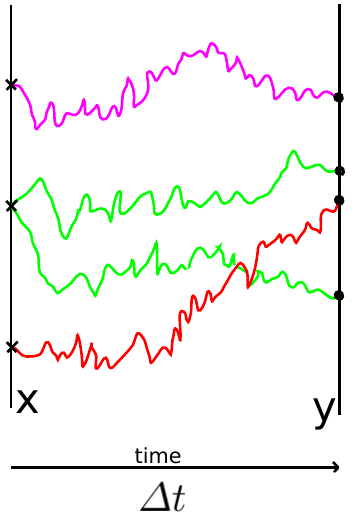
\includegraphics[scale=0.3]{new_img/trainset.png}}
 %   \subfigure[Validation set]{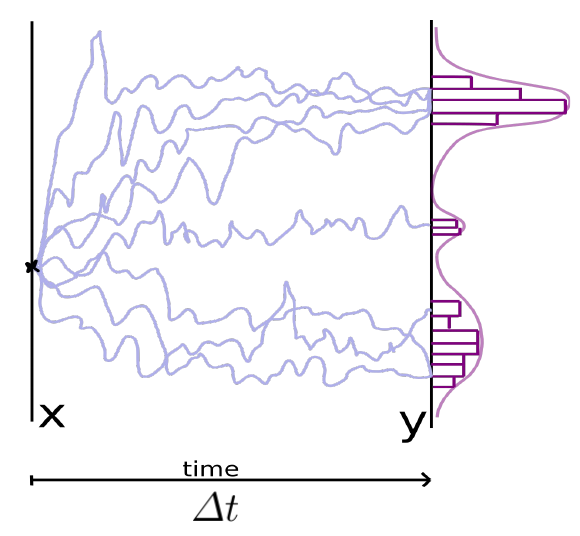
\includegraphics[scale=0.3]{new_img/valset.png}}
%    \caption{Datasets generation}
%    \label{fig:data_gen}
%\end{figure}

\paragraph{Training set. } Choose $n$ random initial states and $n$ parameters. 
 From each of these states, run one or few trajectories of length $T$.

\paragraph{Validation set.} Choose a large number of different initial settings, pairs state-parameter. From each of these states simulate a very large number of SSA trajectories of length $T$.


\section{Learning the transition kernel}

Given a state $s_0$ and a set of parameters $\theta$, the possible futures after a time $\Delta t$ can be represented as a random variable with distribution $K_{\theta}(s\mid s_0)$ over the state space $\mathcal{S}$. We aim at learning an optimal approximation of the conditional distribution $K_{\theta}(s\mid s_0)$ using a conditional GAN~\cite{mirza2014conditional}.

\paragraph{Dynamics-aware dataset}
Each trajectory present in the dataset may be divided in pairs of subsequent states. 
\begin{center}
    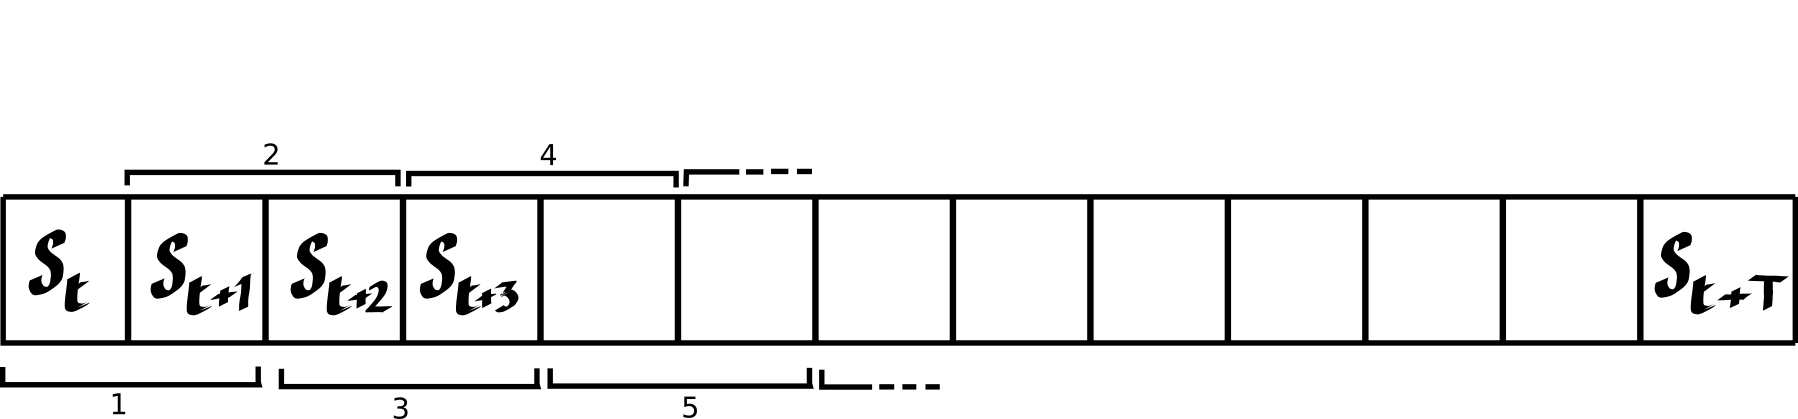
\includegraphics[scale = 0.5]{new_img/trajectory.png}
\end{center}

\paragraph{Conditional Generative Adversarial Nets (c-GAN).} Generative Adversarial Networks, or GANs, are an architecture for training deep learning-based generative models, capable of generating new random plausible examples for a given dataset. Examples can be conditional on a class label or on a continuous variable. However, there is no control over the types of examples that are generated.
The conditional generative adversarial network, or c-GAN for short, is a type of GAN that involves the conditional generation of examples, producing a generator capable of producing examples of a given type.

The architecture is comprised of a generator and a discriminator model. The generator model is responsible for generating new plausible examples that ideally are indistinguishable from real examples in the dataset. The discriminator model is responsible for classifying a given image as either real (drawn from the dataset) or fake (generated).
The models are trained together in a zero-sum or adversarial manner, such that improvements in the discriminator come at the cost of a reduced capability of the generator, and vice versa.

\paragraph{c-GAN architecture.} 
The inputs are states of dimension $d$, which are easier to deal with compared to trajectories, and parameters of dimension $p$. 
The discriminator takes as input  a batch of initial states, $s_0^1,\dots , s_0^b$, a batch of parameters $\theta_1, \dots , \theta_b$, and a batch of subsequent states, $s^1,\dots , s^b$. For each $i\in\{ 1,\dots , b\}$ the inputs, $s_i$, $s_0^i$ and $\theta_i$, are concatenated to form an input with dimension $b\times (2d+p)$. The learning rate is an important parameter to be tuned. The binary cross-entropy is the chosen loss function.

On the other hand, the generator takes as input a batch of initial states, $s_0^1,\dots , s_0^b$, a batch of parameters $\theta_1, \dots , \theta_b$, and a batch of random noise, $z^1,\dots , z^b$, with dimension $k$, a user-defined hyper-parameter. For each $i\in\{ 1,\dots , b\}$ the two inputs are, once again, concatenated to form an input with dimension $b\times (d+p+k)$.

The main advantage, compared to previous approaches, is that c-GANs are very powerful and flexible, capable of learning a multivariate and multimodal conditional distributions without prior knowledge on the shape of such distribution. It is indeed capable of capturing the correlation among different species.

\subsection{Experiments}

\subsubsection{Results: eSIR model with fixed parameters}

\begin{itemize}
    \item $t = 0$:
    \begin{center}
        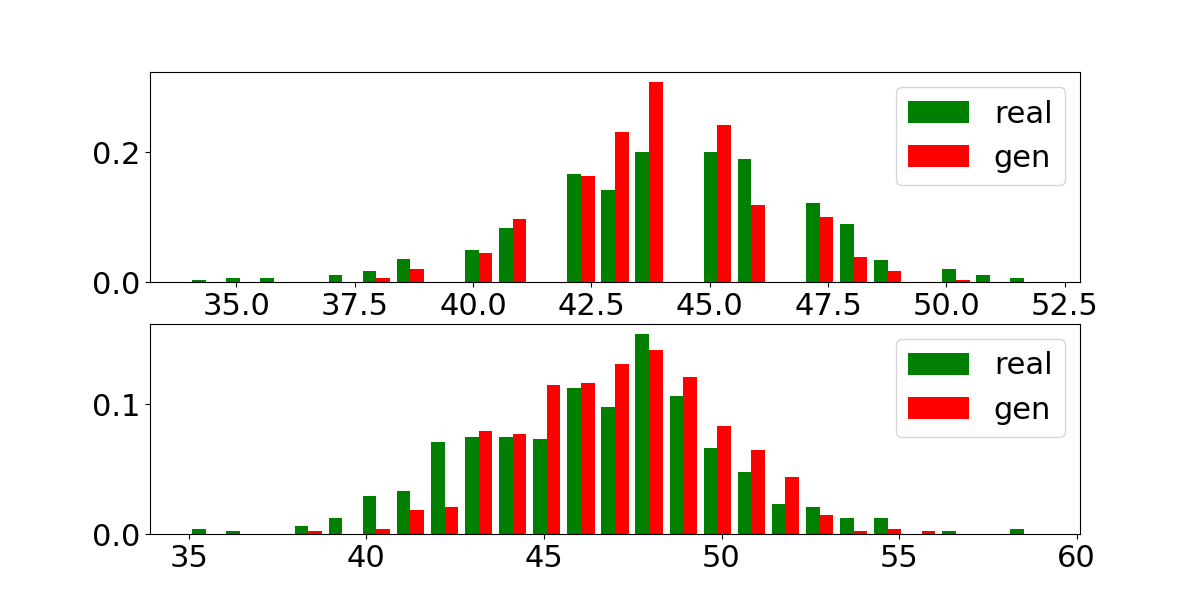
\includegraphics[scale = 0.18]{new_img/eSIR_orig_dataset_hist_comparison_[ 0.04 -0.08]_t_0.png}
        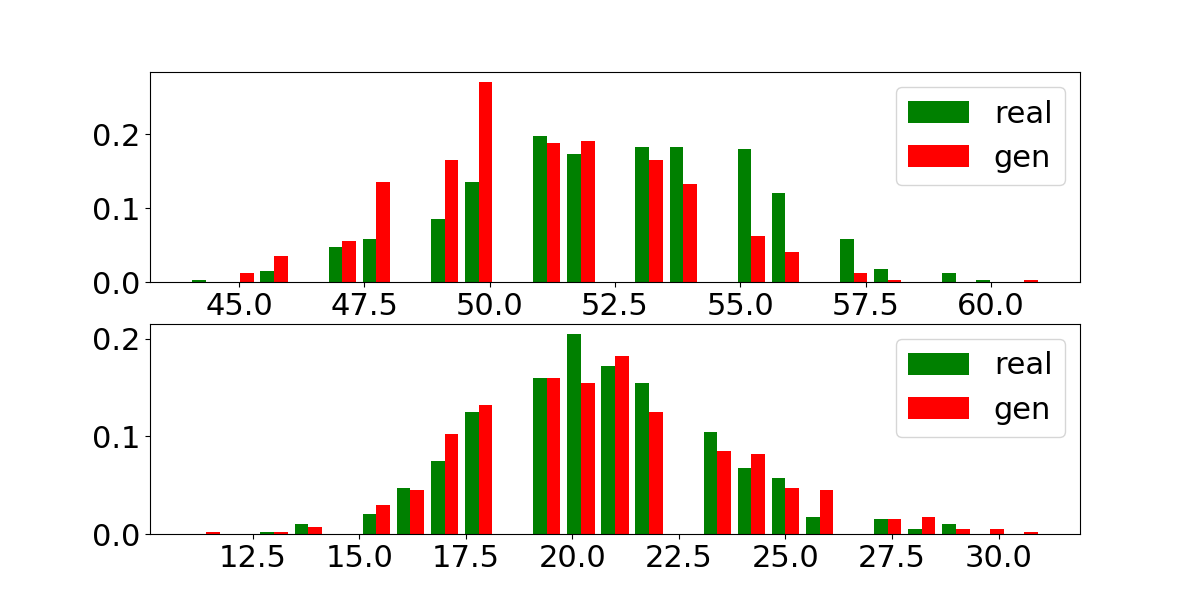
\includegraphics[scale=0.18]{new_img/eSIR_orig_dataset_hist_comparison_[ 0.12 -0.64]_t_0.png}
    \end{center}
    \item $t = 3$:
        \begin{center}
        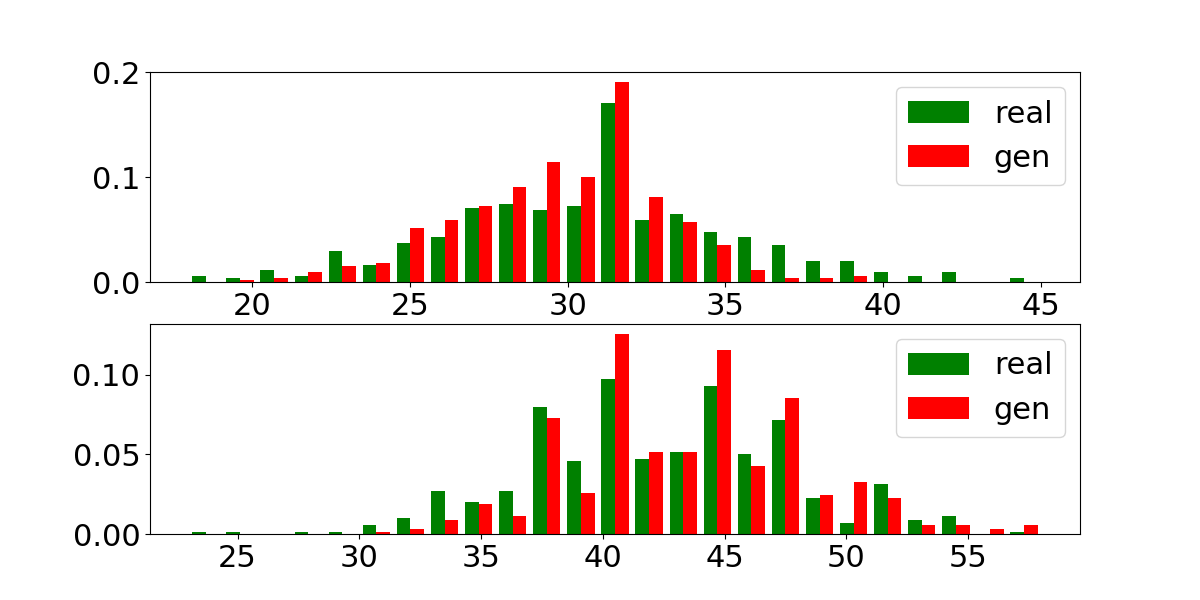
\includegraphics[scale = 0.18]{new_img/eSIR_orig_dataset_hist_comparison_[ 0.04 -0.08]_t_3.png}
        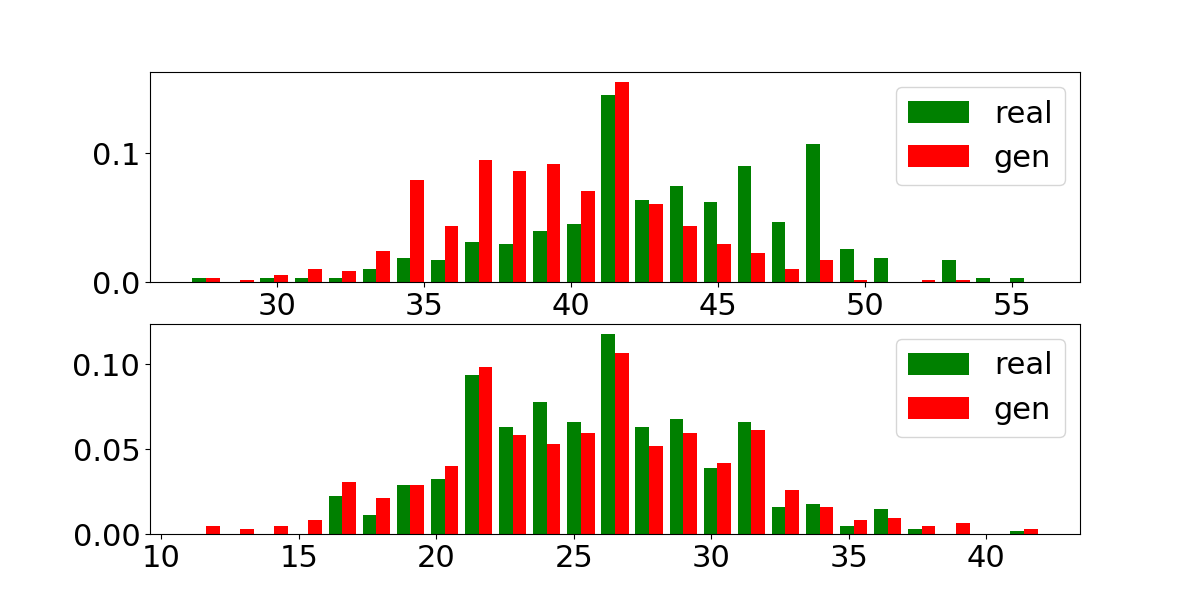
\includegraphics[scale=0.18]{new_img/eSIR_orig_dataset_hist_comparison_[ 0.12 -0.64]_t_3.png}
    \end{center}
    \item $t = 15$:
        \begin{center}
        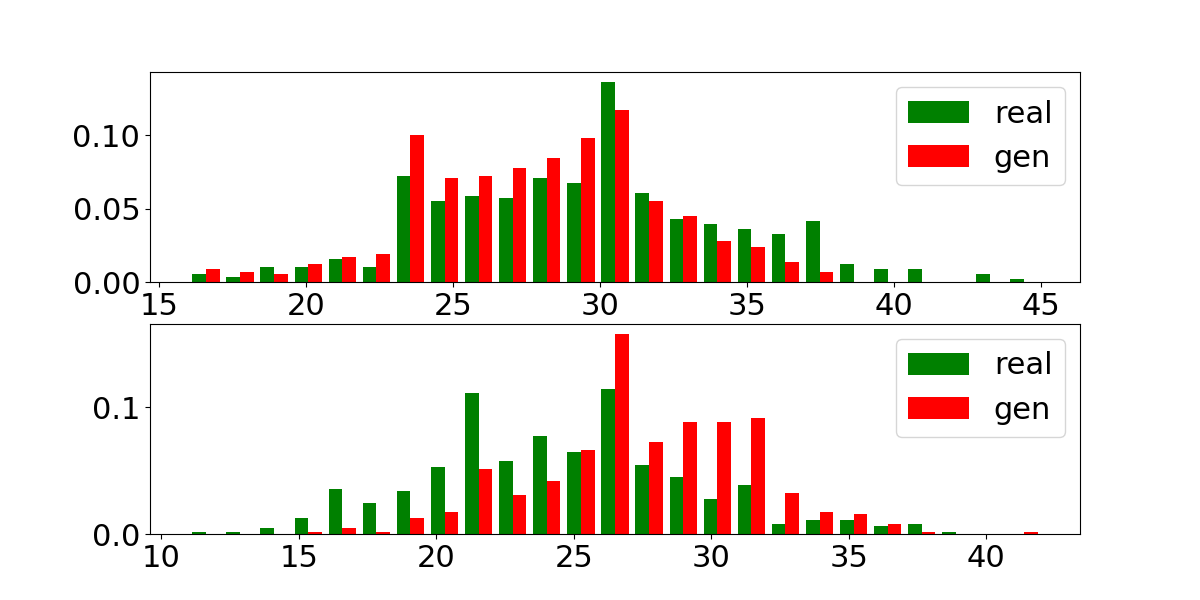
\includegraphics[scale = 0.18]{new_img/eSIR_orig_dataset_hist_comparison_[ 0.04 -0.08]_t_15.png}
        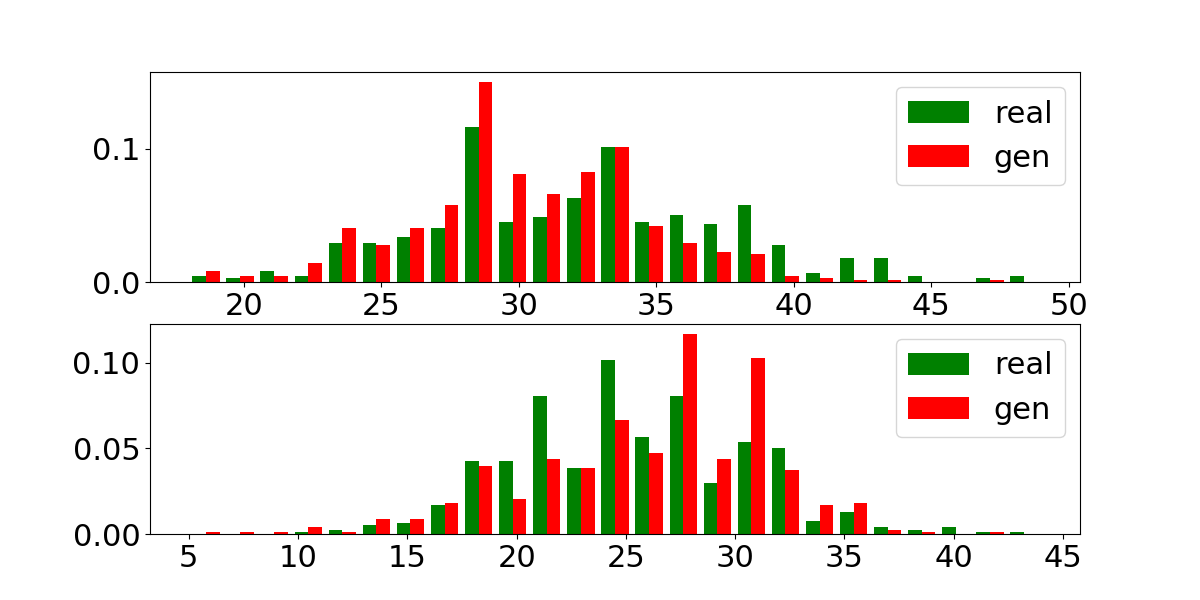
\includegraphics[scale=0.18]{new_img/eSIR_orig_dataset_hist_comparison_[ 0.12 -0.64]_t_15.png}
    \end{center}
    \item $t = 31$:
        \begin{center}
        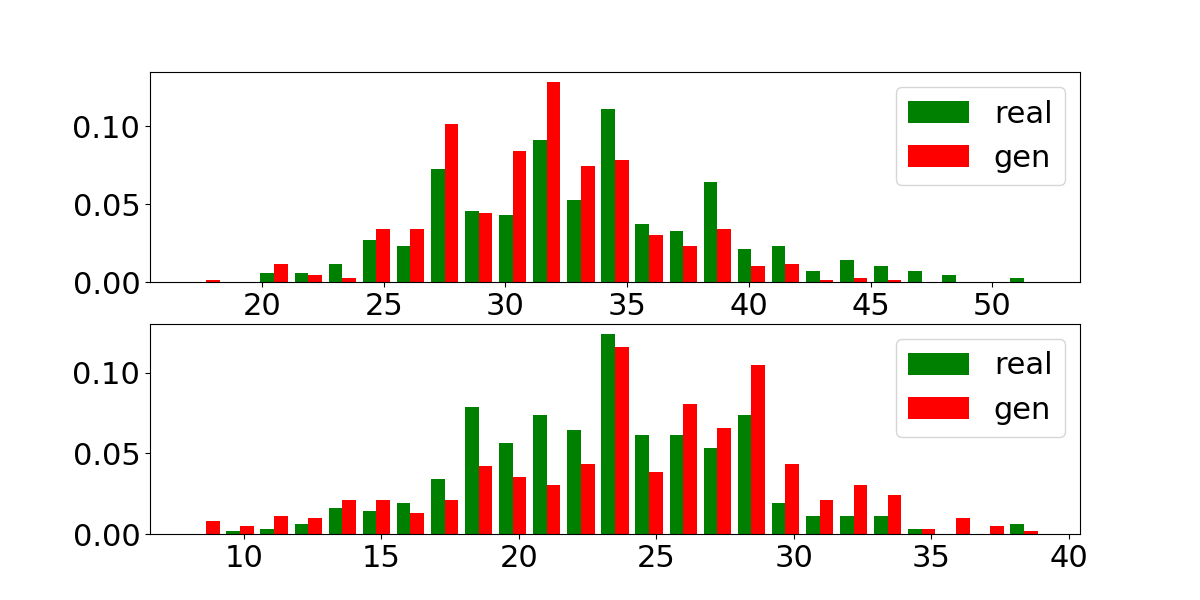
\includegraphics[scale = 0.18]{new_img/eSIR_orig_dataset_hist_comparison_[ 0.04 -0.08]_t_31.png}
        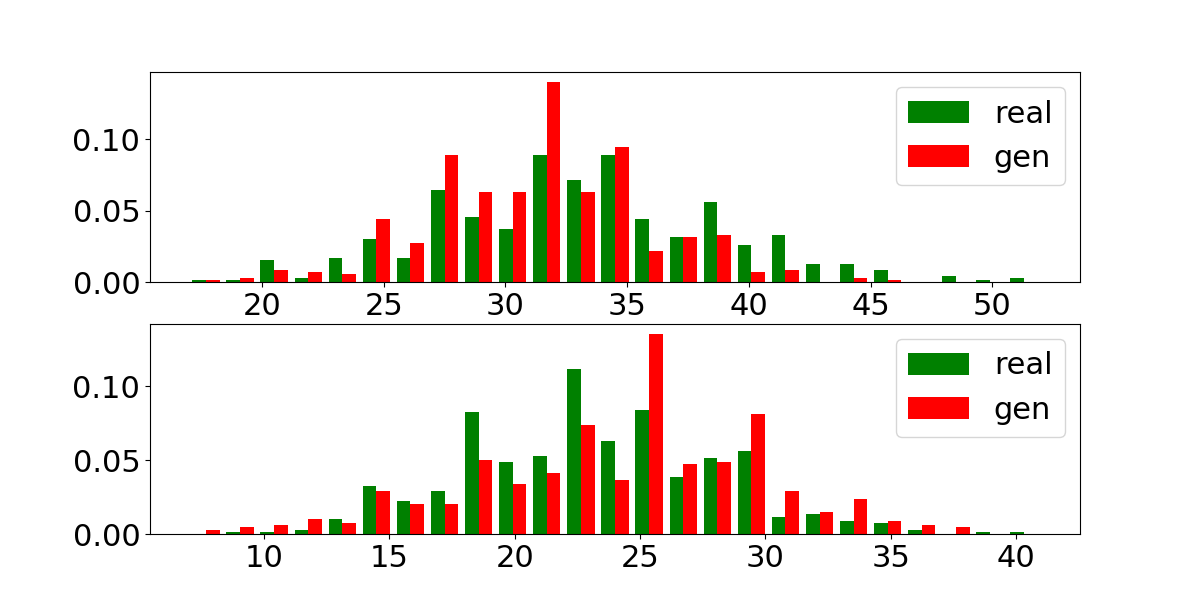
\includegraphics[scale=0.18]{new_img/eSIR_orig_dataset_hist_comparison_[ 0.12 -0.64]_t_31.png}
    \end{center}
\end{itemize}

It is important to analyze wheter the error introduced by the approximation propagates if the abstract kernel is applied iteratively multiple times. The plot below shows the Wasserstein distance, averaged over the entire validation set, among the real and the abstract distribution at each step of iteration.

    \begin{center}
        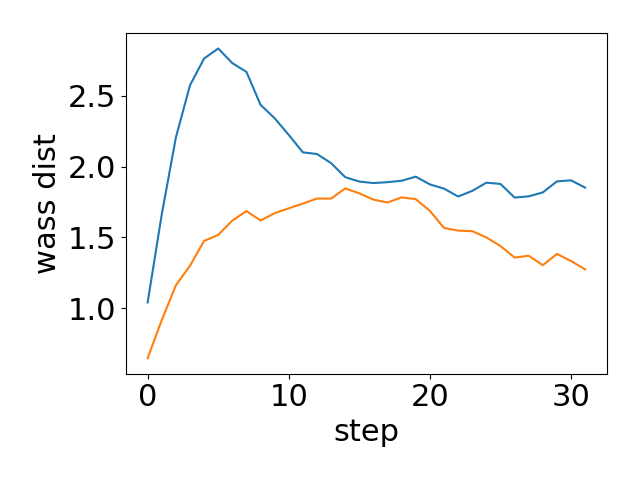
\includegraphics[scale = 0.3]{new_img/eSIR_orig_dataset_avg_wass_distance_32steps.png}
    \end{center}

\subsubsection{TODO}
\begin{itemize}
    \item what about other models? Show results.
    \item  what about the scenario with varying parameters? Show results for eSIR with 1 parameter varying and with 3 parameters varying.
\end{itemize}

\section{Learning to generate a full trajectory}

Given a state $s_0$ and a set of parameters $\theta$, we can be represent the trajectory of length $T$ as a random variable over the state space $\mathcal{S}^T$. Dealing with inputs that are trajectories, i.e. sequences, requires the use of convolutive networks rather than feedforward. 

\paragraph{Wasserstein GAN.} The Wasserstein GAN is an extension to the generative adversarial network that both improves the stability when training the model and provides a loss function that correlates with the quality of generated examples. 
The development of the WGAN has a dense mathematical motivation, although in practice requires only a few minor modifications to the established standard GAN.
In this regard, the Wasserstein GAN (WGAN) seems to work better than a normal GAN, especially regarding the mode collapse behaviour, i.e., when the GAN generates always the same trajectory, missing the stochastic behaviour of the system. 
In particular, the two networks are CNN and the WGAN is conditional. Therefore, we may call it a c-WCGAN (conditional-Wasserstein Convolutional GAN).

The GAN and the WGAN have some important differences that can be specified here (if needed). For example, the discriminator is a binary classifier in the GAN and a regressor, i.e. a critic, in the WGAN.


\paragraph{Differences among GAN and WGAN.} Instead of using a discriminator to classify or predict the probability of generated examples as being real or fake, the WGAN changes or replaces the discriminator model with a critic that scores the realness or fakeness of a given example.
This change is motivated by a theoretical argument that training the generator should seek a minimization of the distance between the distribution of the data observed in the training dataset and the distribution observed in generated examples.
The benefit of the WGAN is that the training process is more stable and less sensitive to model architecture and choice of hyperparameter configurations. Perhaps most importantly, the loss of the discriminator appears to relate to the quality of images created by the generator.

\paragraph{WGAN architecture.} The critic takes as input a trajectory of length $T+1$, as it contains the initial state as well, and it assign a critic value to it. 

TODO: how is the architectural design when we condition on parameters as well? Dense or repeated embedding.

\subsection{Experiments}

\subsubsection{Results: eSIR model with fixed parameters}

The results for the eSIR model are promising and shown in Figure~\ref{fig:esir_trajectories}. Two validation points, i.e., initial states, are chosen. Each point is represented by a pair of trajectories, the top one is for species S and the bottom one is for species I.
\begin{figure}[ht]
    \centering
    \subfigure[]{
    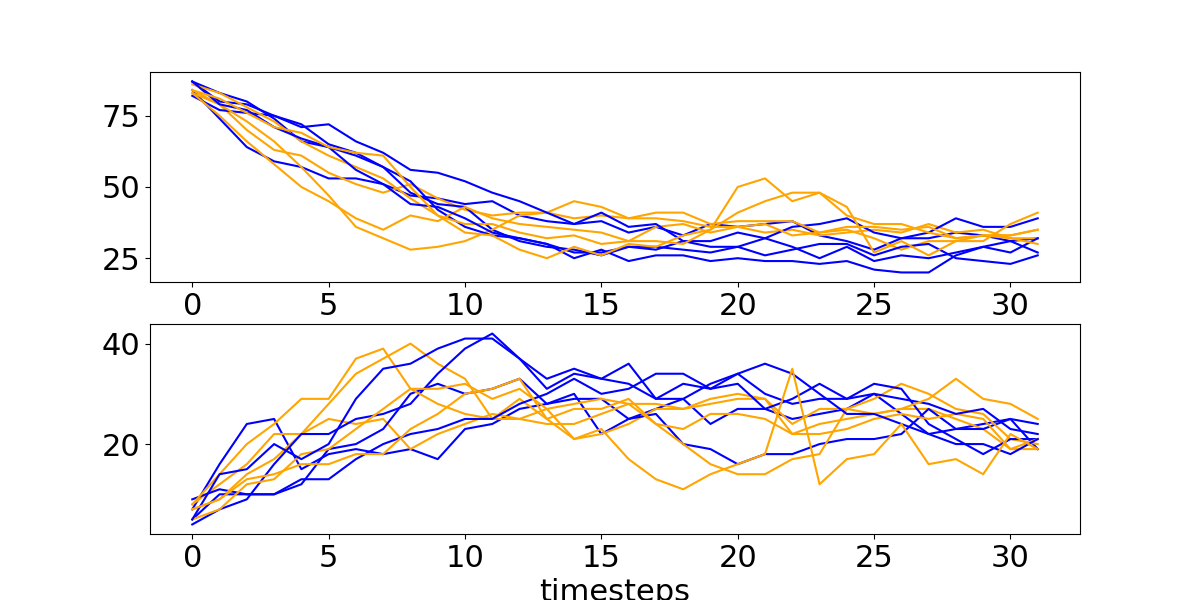
\includegraphics[scale=0.18]{new_img/eSIR_Trajectories4.png}
    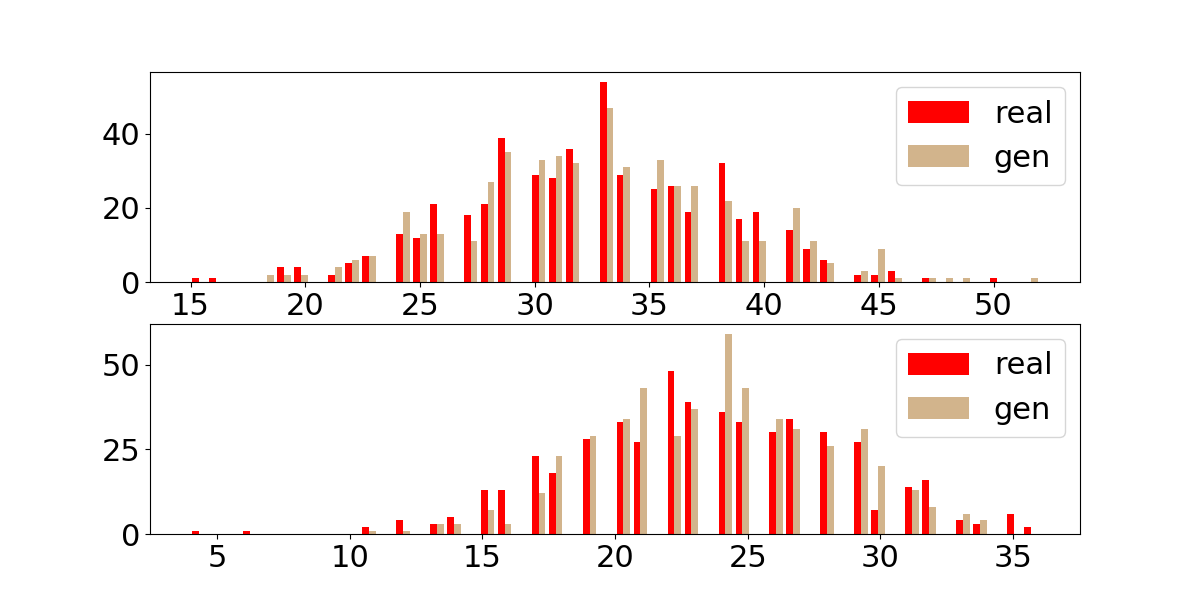
\includegraphics[scale=0.18]{new_img/eSIR_hist_comparison_last_timestep_4.png}
    }
    \subfigure[]{
    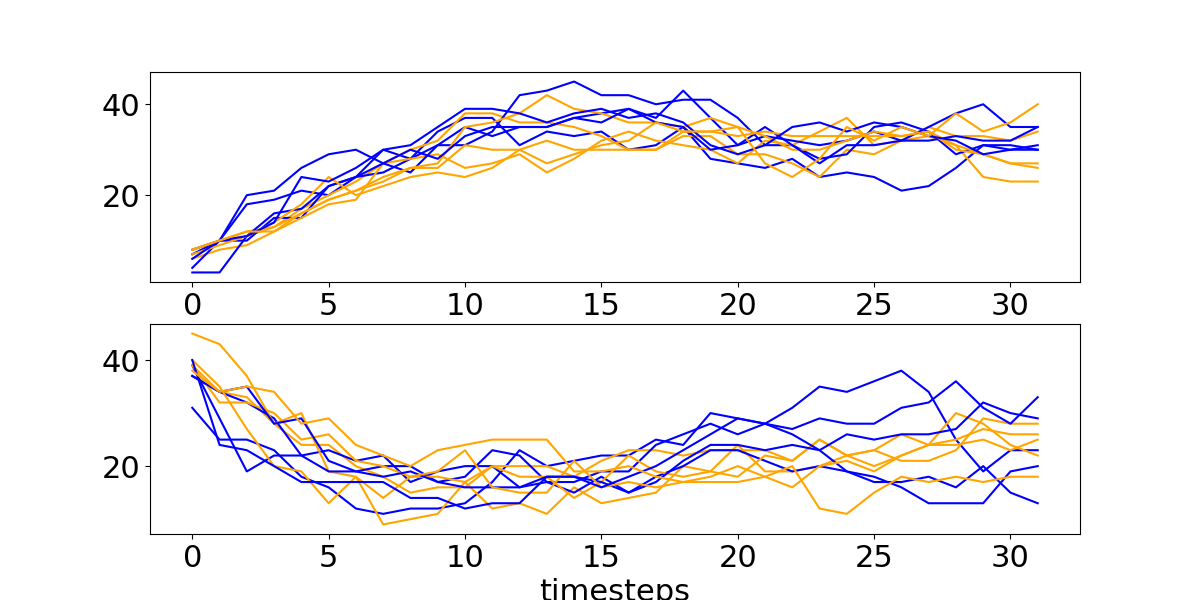
\includegraphics[scale=0.18]{new_img/eSIR_Trajectories8.png}
    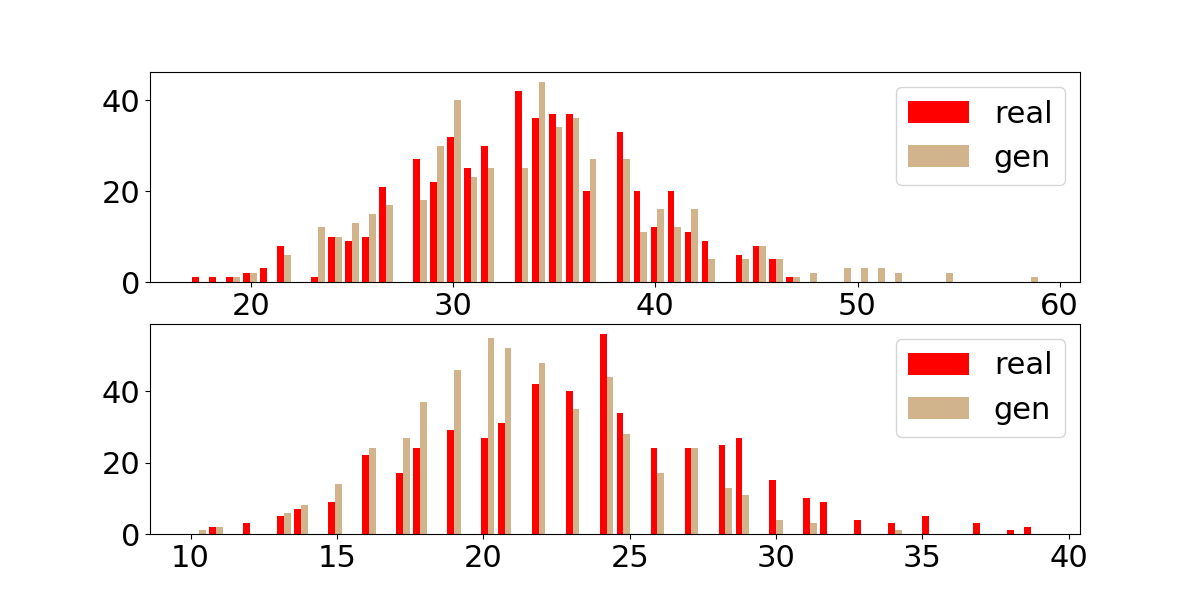
\includegraphics[scale=0.18]{new_img/eSIR_hist_comparison_last_timestep_8.png}
    }
    
    \caption{eSIR model: \textbf{(left)} comparison of trajectories generated with a WGAN (orange) and the trajectories generated with the SSA algorithm (blue); \textbf{(right)} comparison of the real and generated histogram at the last timestep.}
    \label{fig:esir_trajectories}
    \end{figure} 

\paragraph{Measuring error propagation.} Error propagation is measured via the average Wasserstein distance.
\begin{figure}[ht]
    \centering
\subfigure[eSIR]{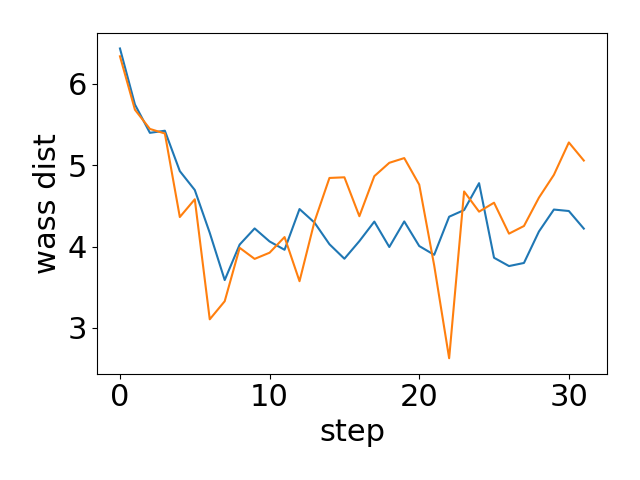
\includegraphics[scale = 0.33]{new_img/eSIR_Traj_avg_wass_distance_200epochs.png}}
\subfigure[eSIR-1 param]{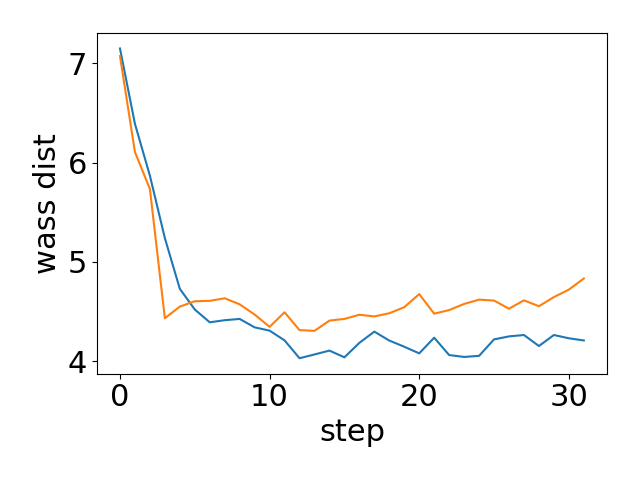
\includegraphics[scale = 0.33]{new_img/ONE_PAR_Traj_avg_wass_distance_200epochs.png}}
\subfigure[Toggle Switch]{  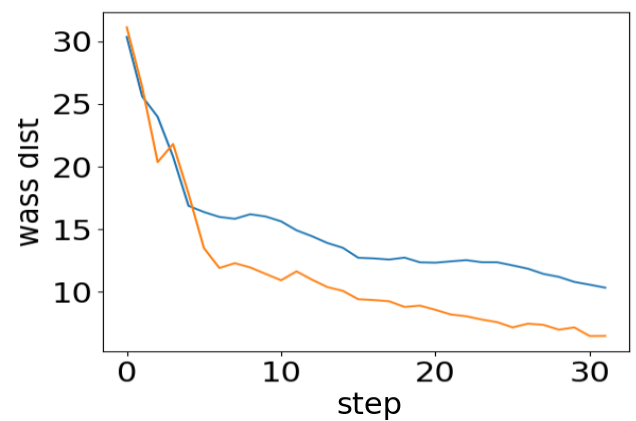
\includegraphics[scale = 0.33]{new_img/TS_avg_wass_distance_400ep.png}}
\subfigure[Repressilator]{  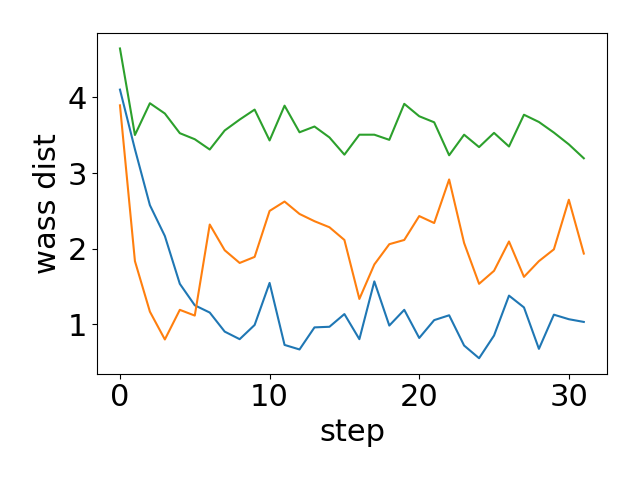
\includegraphics[scale = 0.33]{new_img/Repr_Transient_Traj_avg_wass_distance}}

\end{figure}

%------------------------------

\subsubsection{Results: eSIR model with one parameter varying}

The results for the eSIR model are promising and shown in Figure~\ref{fig:esir_trajectories_one_par}. Four validation points, i.e., initial states, are chosen. Each point is represented by a pair of trajectories, the top one is for species S and the bottom one is for species I.
\begin{figure}[ht]
    \centering
    \subfigure[]{
    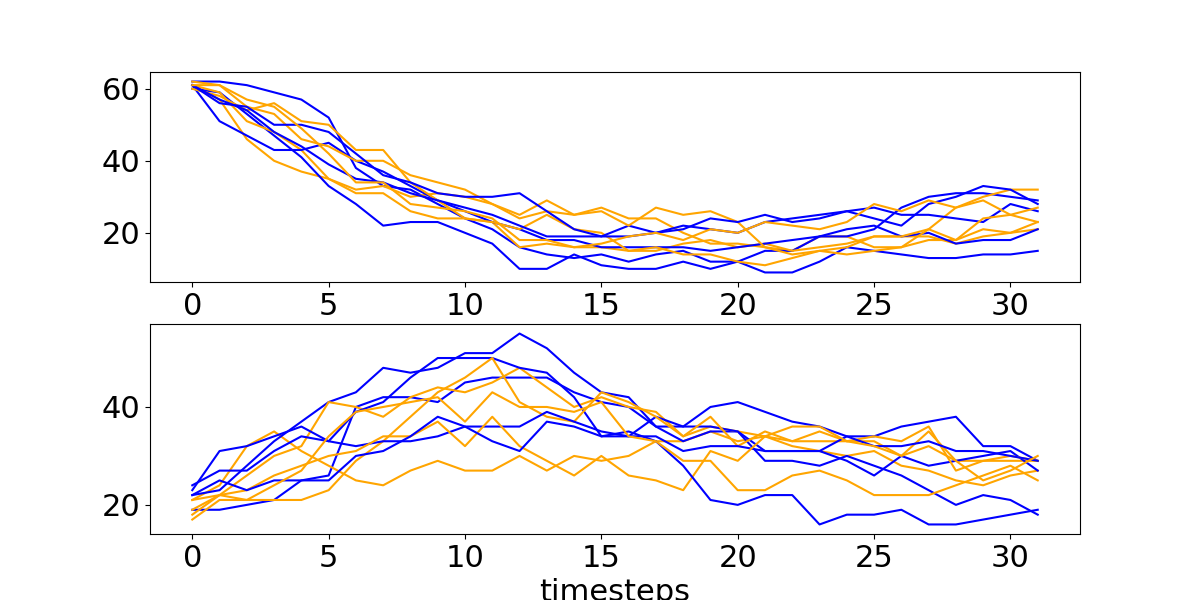
\includegraphics[scale=0.18]{new_img/eSIR_1P_Trajectories0.png}
    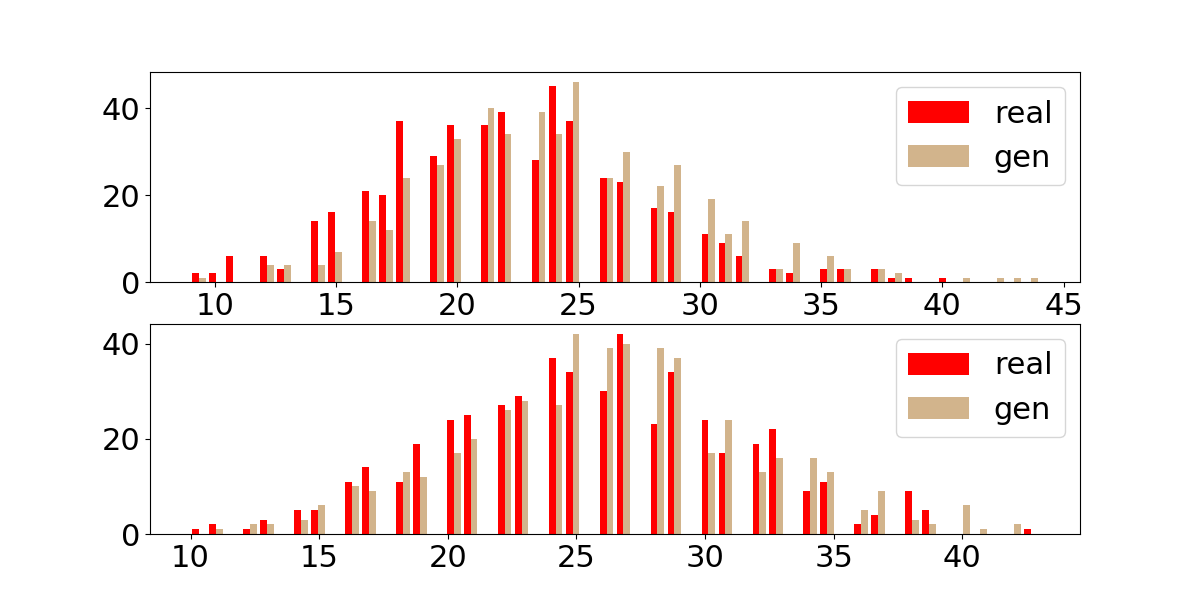
\includegraphics[scale=0.18]{new_img/eSIR_1P_hist_comparison_susc_last_timestep_0.png}
    }
 \subfigure[]{
    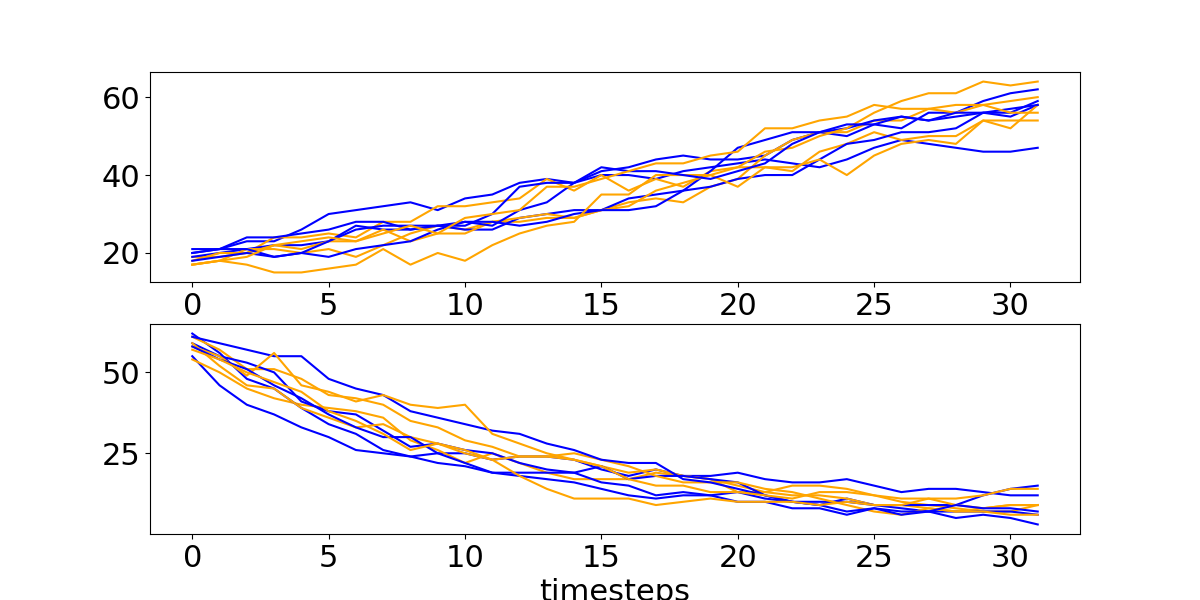
\includegraphics[scale=0.18]{new_img/eSIR_1P_Trajectories1.png}
    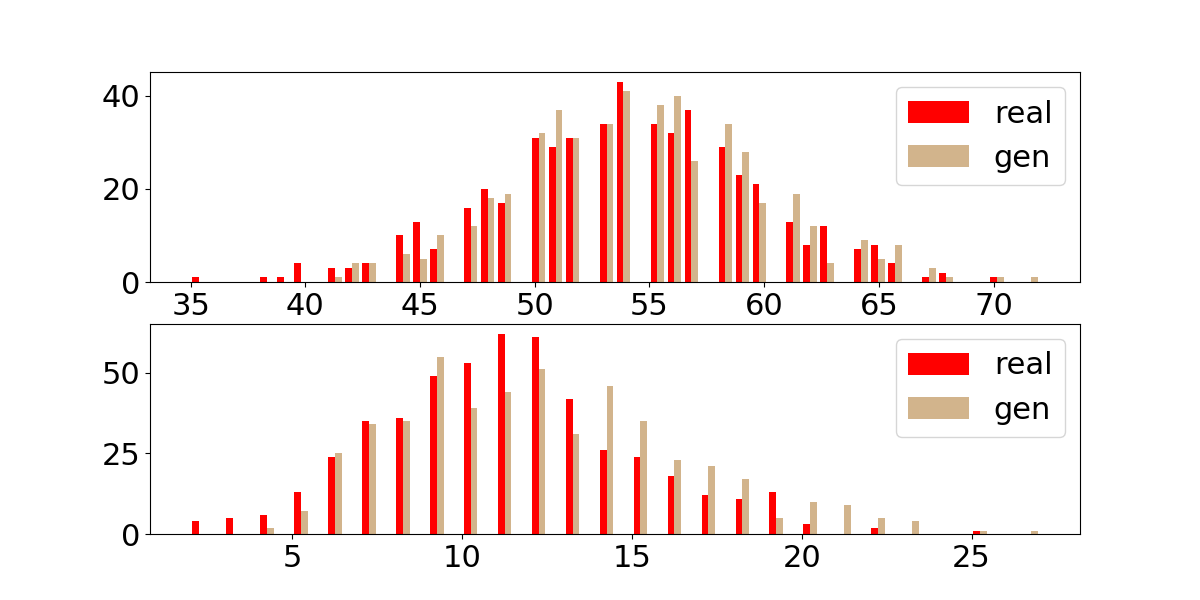
\includegraphics[scale=0.18]{new_img/eSIR_1P_hist_comparison_susc_last_timestep_1.png}
    }
     \subfigure[]{
    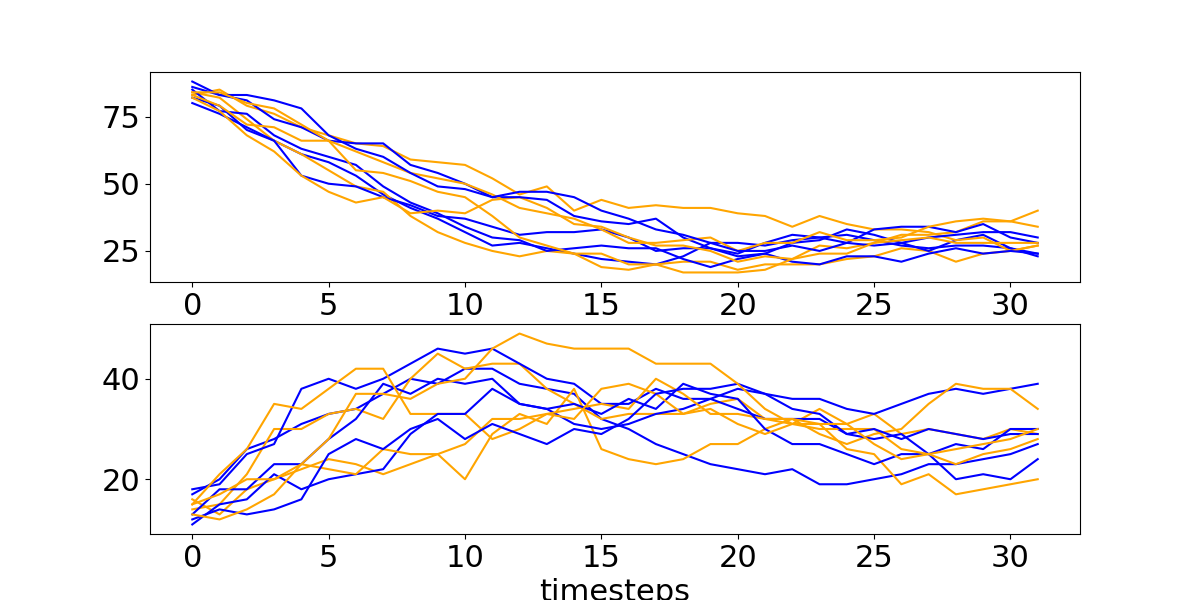
\includegraphics[scale=0.18]{new_img/eSIR_1P_Trajectories2.png}
    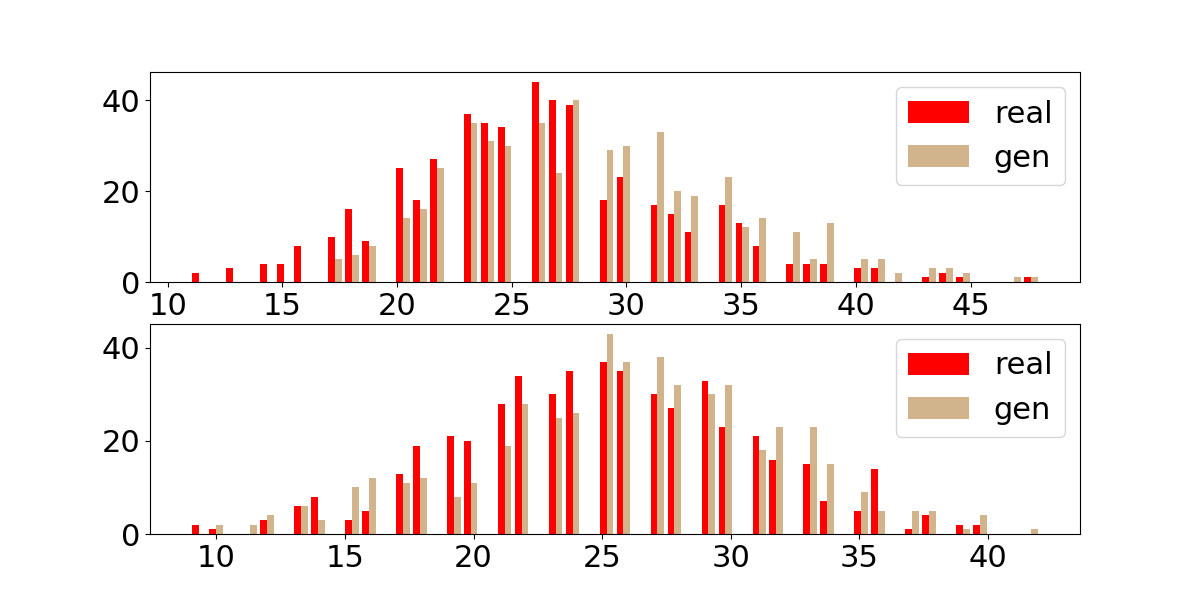
\includegraphics[scale=0.18]{new_img/eSIR_1P_hist_comparison_susc_last_timestep_2.png}
    }
     \subfigure[]{
    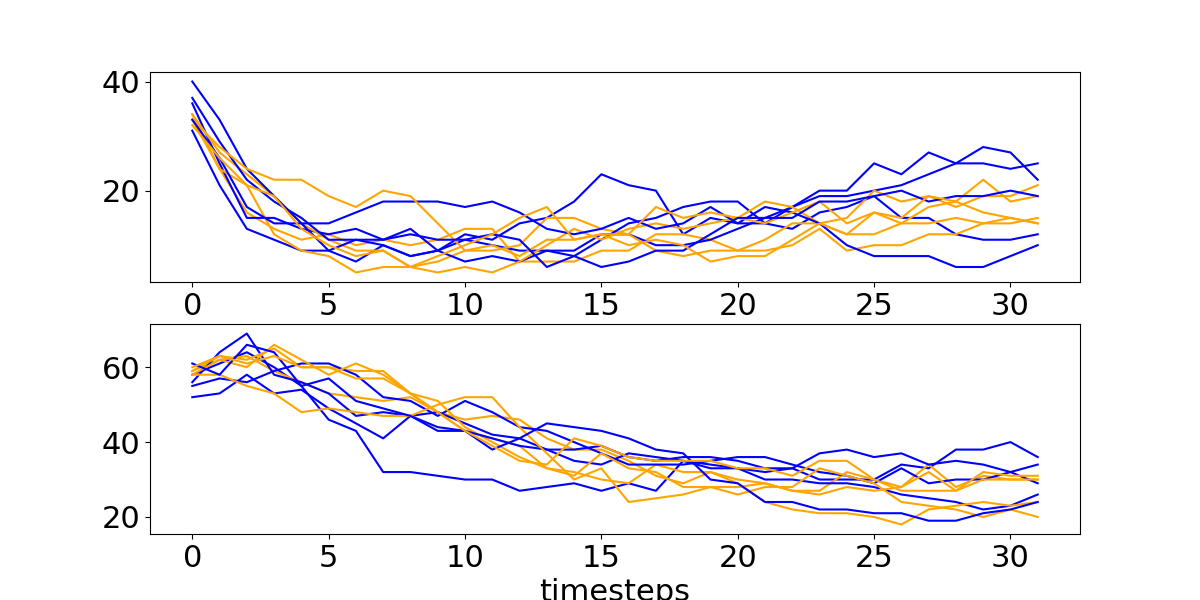
\includegraphics[scale=0.18]{new_img/eSIR_1P_Trajectories4.png}
    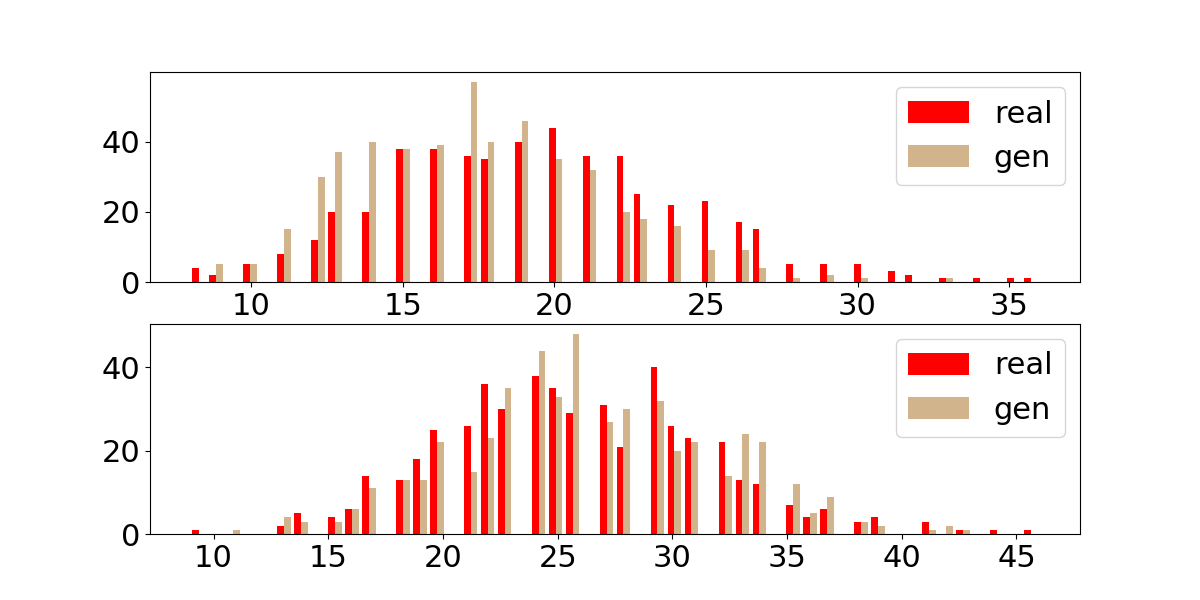
\includegraphics[scale=0.18]{new_img/eSIR_1P_hist_comparison_susc_last_timestep_4.png}
    }
    
    \caption{eSIR model with one varying parameter: \textbf{(left)} comparison of trajectories generated with a WGAN (orange) and the trajectories generated with the SSA algorithm (blue); \textbf{(right)} comparison of the real and generated histogram at the last timestep.}
    \label{fig:esir_trajectories}
    \end{figure} 




\subsubsection{Results: Toggle Switch bistable model with fixed parameters}

The results for the TS model are shown in Figure~\ref{fig:ts_trajectories}. The c-WGAN works well on the trajectories of the proteins, i.e., it is able to capture the bistale beahaviour. This means that we are ignoring the state of the genes. If we take them into account the method does not work. Probably harder to learn the binary trajectories.

\begin{figure}[ht]
    \centering
    \subfigure[]{
    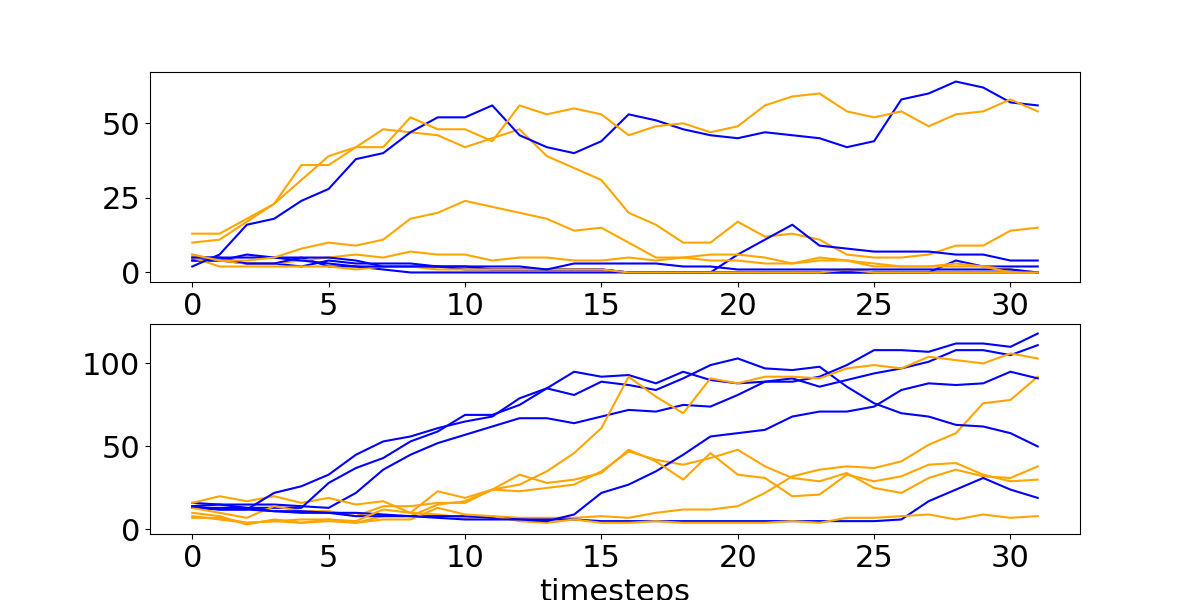
\includegraphics[scale=0.18]{new_img/TS_Trajectories7.png}
    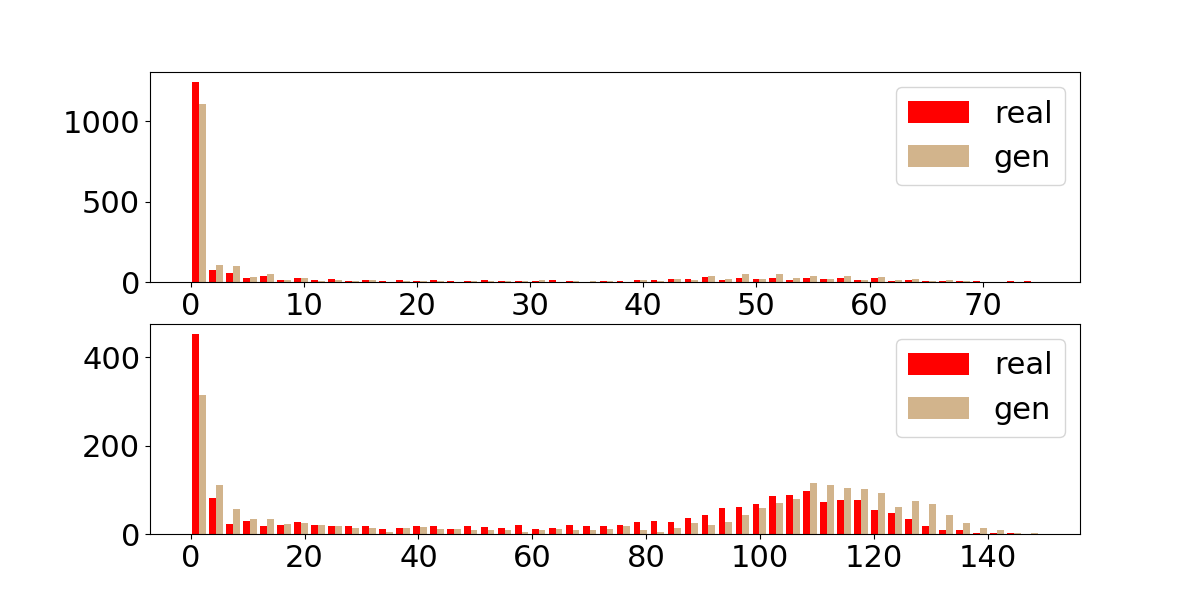
\includegraphics[scale = 0.18]{new_img/TS_hist_comparison_last_timestep_7.png}
    }
    \subfigure[]{
    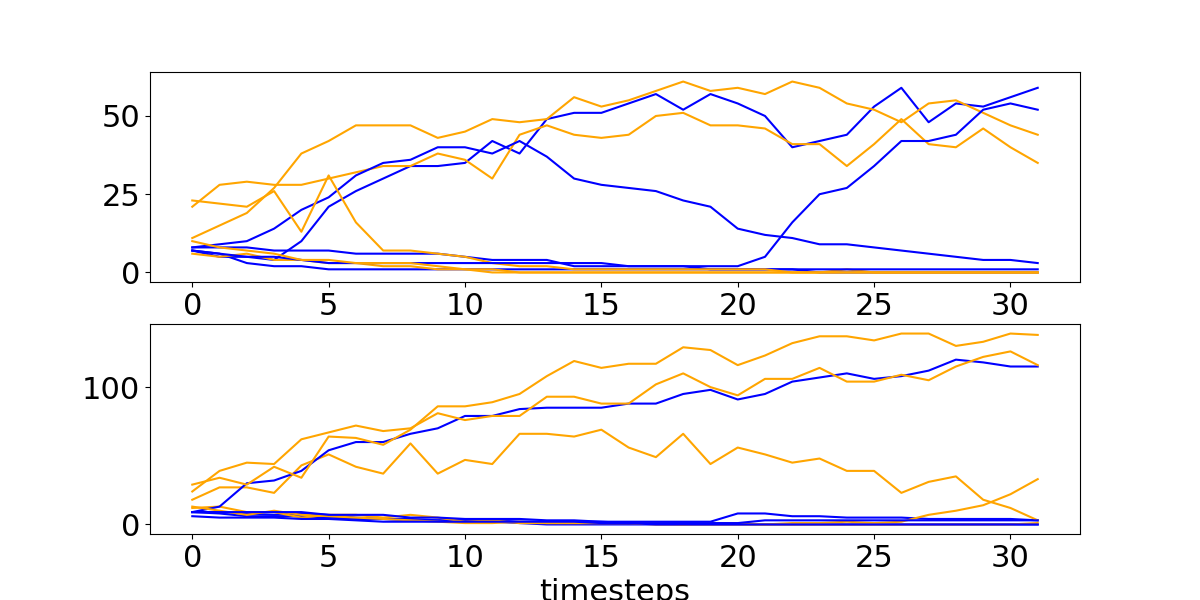
\includegraphics[scale=0.18]{new_img/TS_Trajectories17.png}
    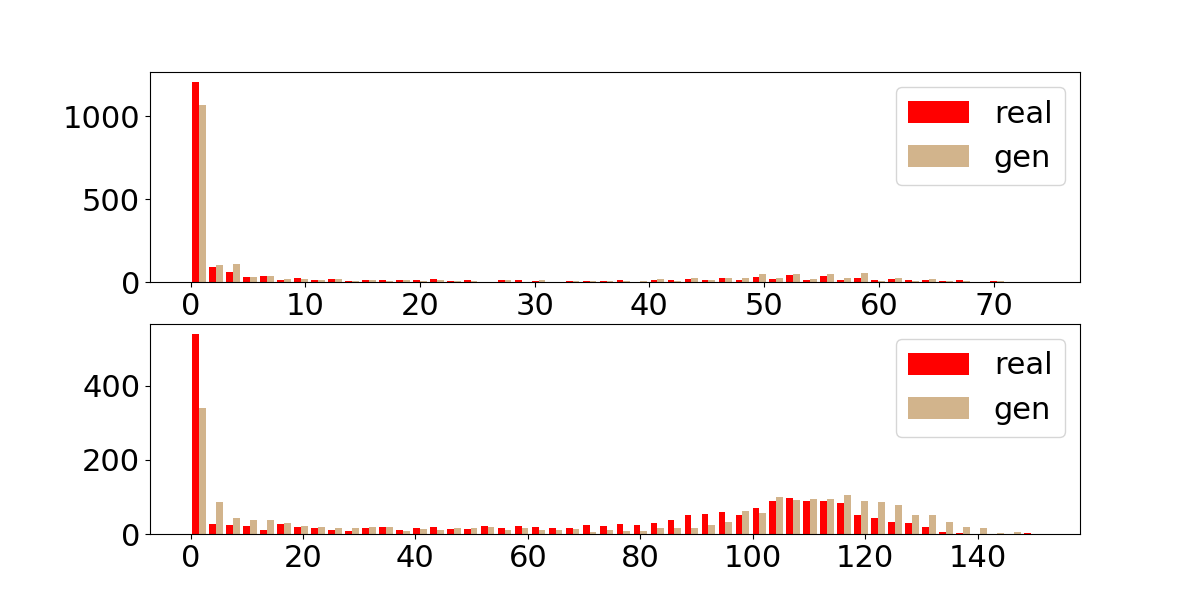
\includegraphics[scale = 0.18]{new_img/TS_hist_comparison_last_timestep_17.png}
    }
    \caption{Toggle Switch model: \textbf{(left)} comparison of trajectories generated with a WGAN (orange) and the trajectories generated with the SSA algorithm (blue); \textbf{(right)} comparison of the real and generated histogram at the last timestep.}
    \label{fig:ts_trajectories}
\end{figure}


\subsubsection{Results: Repressilator oscillating model with fixed parameters}

The results for the Repressilator model are shown in Figure~\ref{fig:repr_trajectories}. The c-WGAN works well on the trajectories of the proteins, i.e., it is able to capture the oscillating beahaviour. Once again, we are ignoring the state of the genes. 

\begin{figure}[ht]
    \centering
    \subfigure[]{
    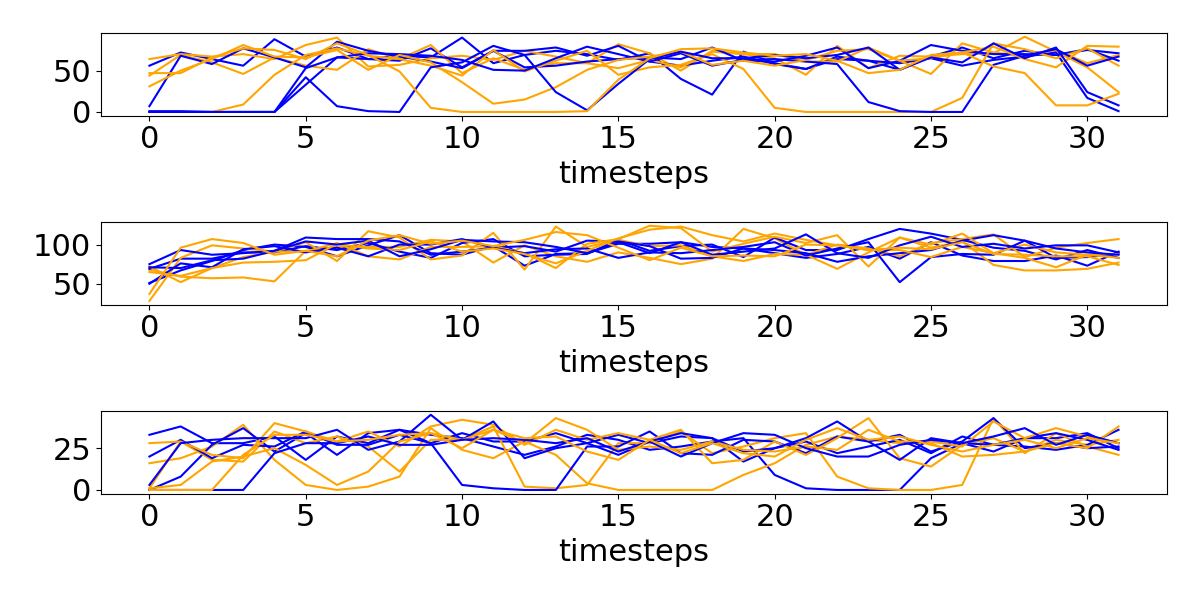
\includegraphics[scale=0.18]{new_img/Repr_Trajectories0.png}
    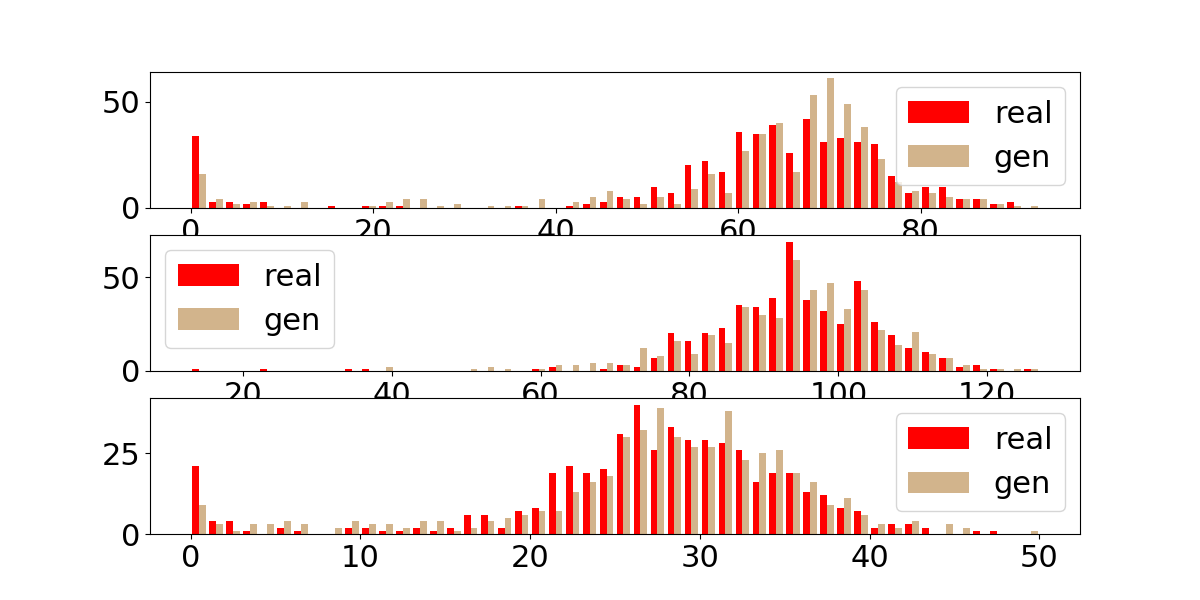
\includegraphics[scale = 0.18]{new_img/Repr_hist_comparison_last_timestep_point_0.png}
    }
    \subfigure[]{
    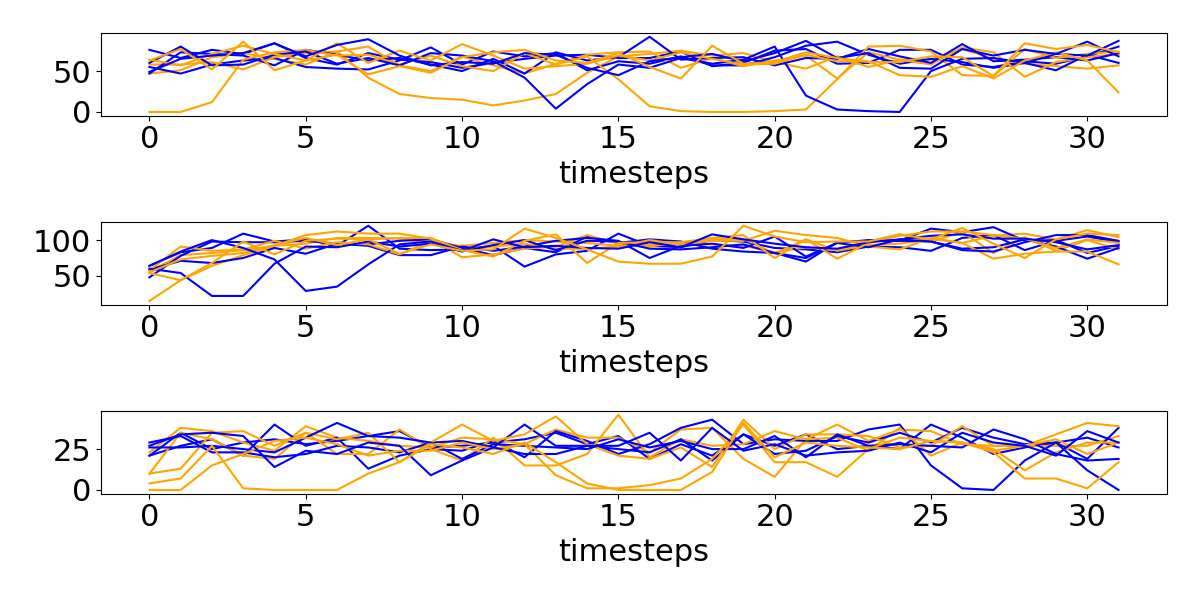
\includegraphics[scale=0.18]{new_img/Repr_Trajectories2.png}
    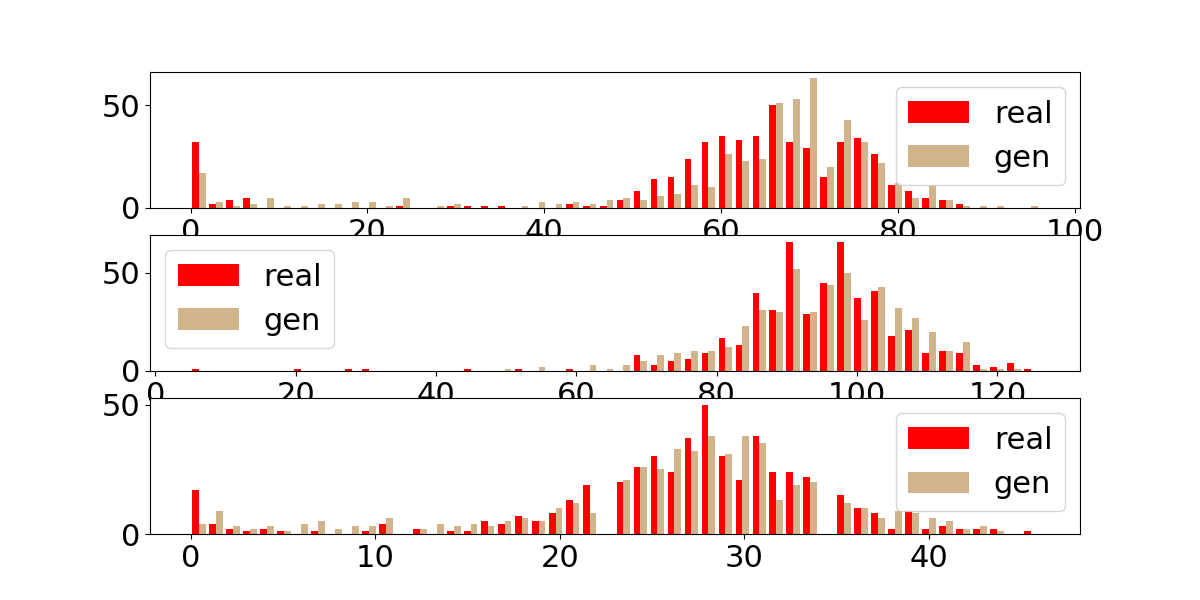
\includegraphics[scale = 0.18]{new_img/Repr_hist_comparison_last_timestep_point_2.png}
    }
    \caption{Repressilator model: \textbf{(left)} comparison of trajectories generated with a WGAN (orange) and the trajectories generated with the SSA algorithm (blue); \textbf{(right)} comparison of the real and generated histogram at the last timestep.}
    \label{fig:repr_trajectories}
\end{figure}





\end{document}
